% Drawing 146/03-4 -- folder 146, batch 03, archive page 57 (PDF page 58).
% Transcription: sous un trait horizontal, deux sphères. À gauche, « I », avec le schéma de trois branches « $\vee\!\!\!\perp\!\vee$ » : équateur à cinq sommets cerclés, coupé par deux grands cercles méridiens ; « $\mathbb{Z}/2$ » ; légende « $9 = 5 + 4$ sommets, \struck{\ill{}} faces, deux cercles marqués » et « $12.5 = 60$ possibilités pour $K$ (pentagone + sommet) », « $D_{01}$ ». À droite, « II », schéma « $\vee\!\!\perp\!\vee$ » : équateur à cinq sommets cerclés, un méridien ; « $\mathbb{Z}/2$ » ; légende « $5 + 2 = 7$ sommets, 4 faces, 1 cercle marqué » et « $12.5 = 60$ poss.\ \uncertain{pour} \ill{} (pentagone + arête) », « $D_{02}$ ».
% Kind: cell decomposition of the sphere (two cases). Method 3 (encoded, rendered from the data). Status: ok.
% Notes: I: equator with five ringed vertices cut by two disjoint marked circles (each meets the equator twice): encoded V=9 (5+4, as he writes), E=13, F=6 -- his face count is struck and illegible, the encoding gives 6. II: equator with five ringed vertices and one marked meridian: V=7, F=4 as he writes. The three-branch schemas are given as text (as in the transcription), not redrawn stroke by stroke. Exact order of the crossings among the ringed vertices read from the figure; it does not affect the counts.
% Coordinates: 1 unit = 1 mm = 1/100 of the crop width (bbox in page fractions: [0.1, 0.57, 0.88, 0.87]).
% Redrawn by Claude (claude-opus-5-5), issue #73 pilot, 2026-11-07; not checked by a human; not compiled (no TeX in the session).
% Rights: reproduces part of the work -- behind RENDER_TRANSCRIPTS, never published by itself.
\documentclass[tikz,border=3pt]{standalone}
\usepackage{amsmath,amssymb}
\usetikzlibrary{patterns,arrows.meta}
\tikzset{pencil/.style={black!45}, struck/.style={black!35}, mark/.style={circle,draw,inner sep=1.3pt}, pt/.style={circle,fill,inner sep=0.9pt}, opt/.style={circle,draw,fill=white,inner sep=1.1pt}}
\begin{document}
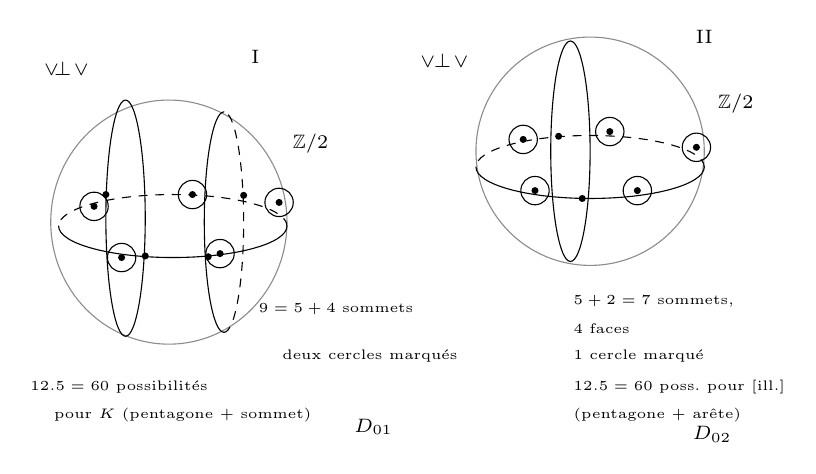
\begin{tikzpicture}[x=1mm,y=1mm,line cap=round,line join=round,font=\scriptsize]
\draw[pencil] (24,-26) ellipse[x radius=15, y radius=15.5];
\draw[dashed] (39,-26.5) arc[start angle=0, end angle=180, x radius=14.5, y radius=4];
\draw (10,-26.5) arc[start angle=180, end angle=360, x radius=14.5, y radius=4];
\draw (18.5,-25.5) ellipse[x radius=2.5, y radius=15];
\draw (31,-12) arc[start angle=90, end angle=270, x radius=2.5, y radius=14];
\draw[dashed] (31,-40) arc[start angle=-90, end angle=90, x radius=2.5, y radius=14];
\draw (14.5,-24) circle[radius=1.8];
\draw (27,-22.5) circle[radius=1.8];
\draw (38,-23.5) circle[radius=1.8];
\draw (18,-30.5) circle[radius=1.8];
\draw (30.5,-30) circle[radius=1.8];
\node[pt] at (14.5,-24) {};
\node[pt] at (27,-22.5) {};
\node[pt] at (38,-23.5) {};
\node[pt] at (18,-30.5) {};
\node[pt] at (30.5,-30) {};
\node[pt] at (16,-22.5) {};
\node[pt] at (21,-30.3) {};
\node[pt] at (29,-30.4) {};
\node[pt] at (33.5,-22.6) {};
\node[inner sep=1pt] at (11,-6.5) {\scriptsize $\vee\!\!\!\perp\!\vee$};
\node[inner sep=1pt] at (35,-5) {\scriptsize I};
\node[inner sep=1pt] at (42,-16) {\scriptsize $\mathbb{Z}/2$};
\node[inner sep=1pt,anchor=west] at (35,-37) {\tiny $9=5+4$ sommets};
\node[inner sep=1pt,anchor=west] at (38,-43) {\tiny deux cercles marqués};
\node[inner sep=1pt,anchor=west] at (6,-47) {\tiny $12.5=60$ possibilités};
\node[inner sep=1pt,anchor=west] at (9,-50.5) {\tiny pour $K$ (pentagone + sommet)};
\node[inner sep=1pt] at (50,-52) {\scriptsize $D_{01}$};
\draw[pencil] (77.5,-17) ellipse[x radius=14.5, y radius=14.5];
\draw[dashed] (92,-19) arc[start angle=0, end angle=180, x radius=14.5, y radius=4];
\draw (63,-19) arc[start angle=180, end angle=360, x radius=14.5, y radius=4];
\draw (75,-17) ellipse[x radius=2.5, y radius=14];
\draw (69,-15.5) circle[radius=1.8];
\draw (80,-14.5) circle[radius=1.8];
\draw (91,-16.5) circle[radius=1.8];
\draw (70.5,-22) circle[radius=1.8];
\draw (83.5,-22) circle[radius=1.8];
\node[pt] at (69,-15.5) {};
\node[pt] at (80,-14.5) {};
\node[pt] at (91,-16.5) {};
\node[pt] at (70.5,-22) {};
\node[pt] at (83.5,-22) {};
\node[pt] at (73.5,-15.1) {};
\node[pt] at (76.5,-23) {};
\node[inner sep=1pt] at (59,-5.5) {\scriptsize $\vee\!\!\perp\!\vee$};
\node[inner sep=1pt] at (92,-2.5) {\scriptsize II};
\node[inner sep=1pt] at (96,-11) {\scriptsize $\mathbb{Z}/2$};
\node[inner sep=1pt,anchor=west] at (75,-36) {\tiny $5+2=7$ sommets,};
\node[inner sep=1pt,anchor=west] at (75,-39.5) {\tiny 4 faces};
\node[inner sep=1pt,anchor=west] at (75,-43) {\tiny 1 cercle marqué};
\node[inner sep=1pt,anchor=west] at (75,-47) {\tiny $12.5=60$ poss.\ pour [ill.]};
\node[inner sep=1pt,anchor=west] at (75,-50.5) {\tiny (pentagone + arête)};
\node[inner sep=1pt] at (93,-53) {\scriptsize $D_{02}$};
\end{tikzpicture}
\end{document}
